\documentclass[11pt,a4paper]{article}

\usepackage{amsmath}
\usepackage{amsfonts}
\usepackage{amssymb}
\usepackage{graphicx}
\usepackage{float}
\usepackage[left=1in,right=1in,top=1in,bottom=1in]{geometry}

\title{Machine Learning in Complex Domains:\\Assignment 3}
\author{Ryan Cotterell, Daniel Deutsch, Dan Crankshaw}
\date{}

\begin{document}

	\maketitle
	
	\setcounter{section}{3}
	\section{Blocked Gibbs Sampler}
	
	\subsection{Analysis Questions}


        We have the following equation
$$
p(z_{d,i} = k,x_{d,i} = c| \mathbf{z} - z_{d,i},\mathbf{x} - x_{d,i}, \mathbf{c},\mathbf{w} ; \alpha,\beta,\lambda) = \frac{p(\mathbf{z},\mathbf{x},\mathbf{c},\mathbf{w}|\alpha,\beta,\lambda)}{p(\mathbf{z} - z_{d,i},\mathbf{x} - x_{d,i},\mathbf{c},\mathbf{w} ; \alpha,\beta,\lambda)}
$$
The full join (numerator) is given to us in the assignment. We can factor this according to the joint and every term that does not involve $z_{d,i}$ or $x_{d,i}$ will cancel. This is basically a union of (15) and (18). This yields the following:
$$
p(z_{d,i} = k, x_{d,i} = 0| \mathbf{z} - z_{d,i},\mathbf{x} - x_{d,i}, \mathbf{c},\mathbf{w} ; \alpha,\beta,\lambda) = \frac{p(x=0|\lambda)
  \frac{\Gamma(n^k_{w_{d,i}} + 1 + \beta)}{\Gamma(1 + \sum_w n_w^k + \beta )} 
    \frac{\Gamma(n_k^d + 1 + \alpha)}{\Gamma(1 + \sum_{k'} n_{k'}^d + \alpha)}
    }
    {
    \frac{\Gamma(n_{w_{d,i}}^k + \beta)}{\Gamma(\sum_w n_w^k + \beta )}
    \frac{\Gamma(n_k^d + \alpha)}{\Gamma(\sum_{k'} n_{k'}^d + \alpha) } 
    }
$$
$$
p(z_{d,i} = k, x_{d,i} = 0| \mathbf{z} - z_{d,i},\mathbf{x} - x_{d,i}, \mathbf{c},\mathbf{w} ; \alpha,\beta,\lambda) \propto \frac{(1-\lambda) (n_{w_{d,i}}^k + \beta) (n_k^d + \alpha)}{(n_*^k + K\beta)(n_*^d + V\alpha)}
$$
By analogy, we get the followoing for the case that $p(x=1)$. 
$$
p(z_{d,i} = k, x_{d,i} = 1| \mathbf{z} - z_{d,i},\mathbf{x} - x_{d,i}, \mathbf{c},\mathbf{w} ; \alpha,\beta,\lambda) \propto \frac{\lambda (n_{w_{d,i}}^k + \beta) (n_k^d + \alpha)}{(n_*^k + K\beta)(n_*^d + V\alpha)}
$$
Most of the heavy lifting for this question was done in the appendix so there isn't really any more we can write. 

	
	\section{Text Analysis with MCLDA}
	\subsection{Empirical Questions}
	\begin{enumerate}
		\item On all three chains, the test likelihood is lower than the
		training likelihood by approximately the same amount. By around iteration
		200, the likelihoods have more or less converged, indicating that 
		the Markov chain is sufficiently mixed. Because our topic counts are
		based on the training data, it makes sense that the test likelihood is lower
		than the training likelihood.
			\begin{figure}[H]
				\caption{Question 1}
				\begin{center}
					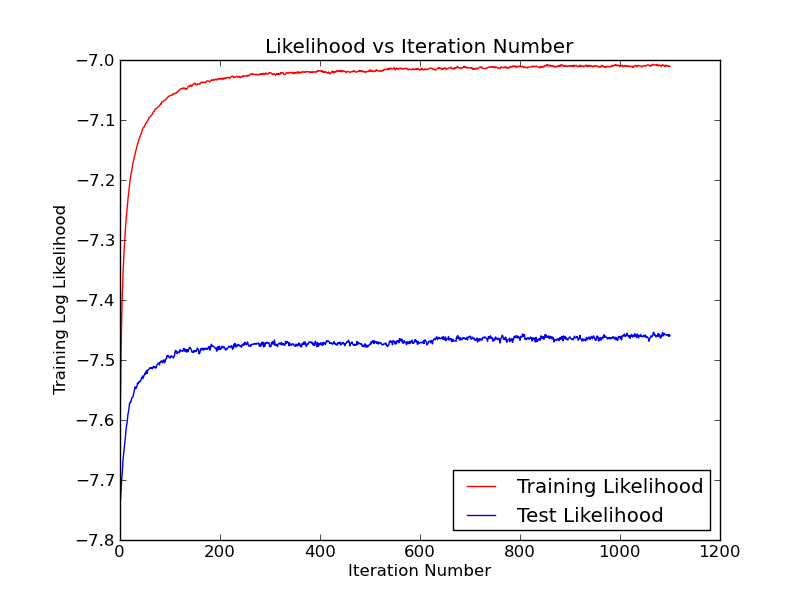
\includegraphics[scale=0.5]{../train_test_1}
				\end{center}
			\end{figure}
			\begin{figure}[H]
				\caption{Question 1}
				\begin{center}
					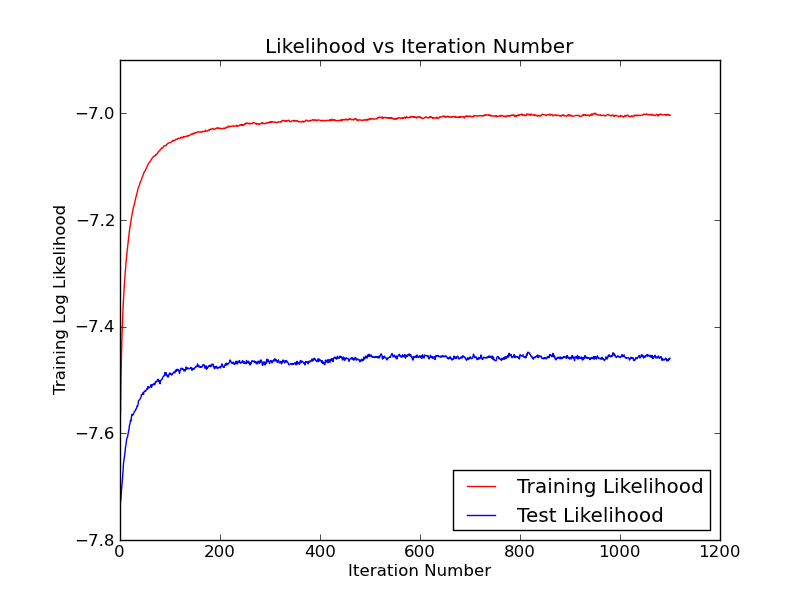
\includegraphics[scale=0.5]{../train_test_2}
				\end{center}
			\end{figure}
			\begin{figure}[H]
				\caption{Question 1}
				\begin{center}
					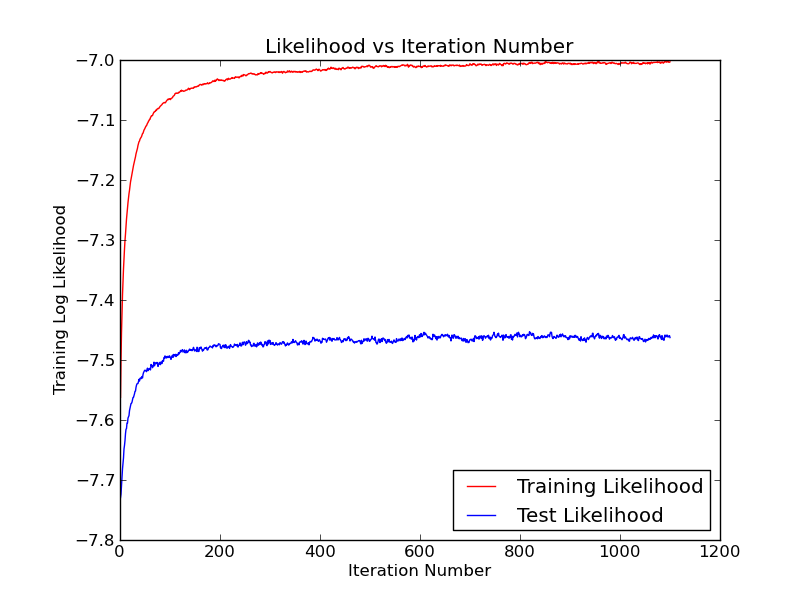
\includegraphics[scale=0.5]{../train_test_3}
				\end{center}
			\end{figure}
			
		\item The collapsed sampler seems to mix about 50-100 iterations
		faster than the blocked sampler. However, the blocked sampler reaches
		a higher final likelihood.

			\begin{figure}[H]
				\caption{Question 2}
				\begin{center}
					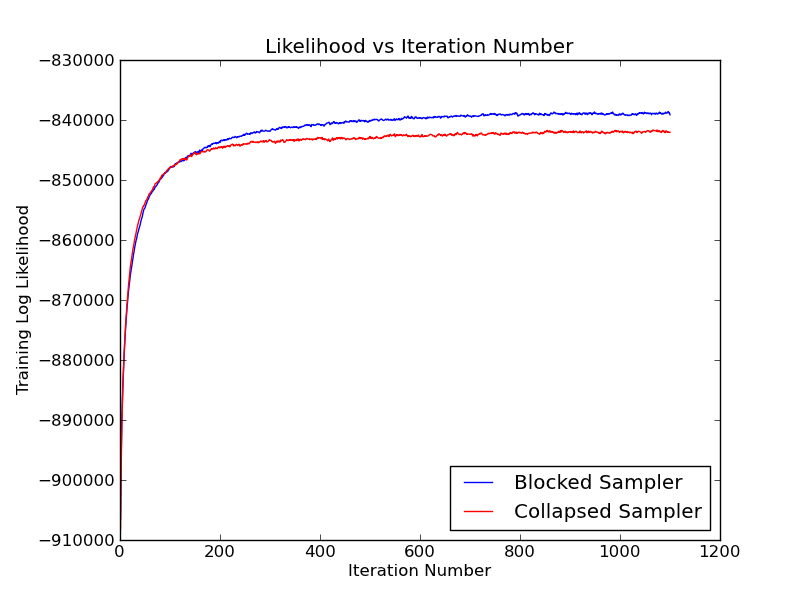
\includegraphics[scale=0.5]{../block_v_collapse_plot}
				\end{center}
			\end{figure}
			
		\item 	
		The average runtime for the blocked iterations was 300ms and for the
		collapsed iteration it was 229ms.
			\begin{figure}[H]
				\caption{Question 3}
				\begin{center}
					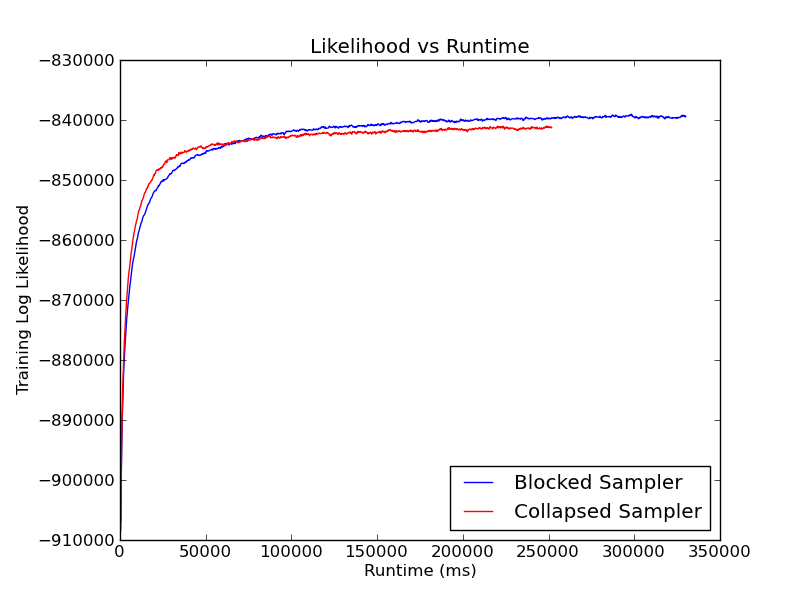
\includegraphics[scale=0.5]{../runtime_plot}
				\end{center}
			\end{figure}
		\item
			\begin{figure}[H]
				\caption{Question 4}
				\begin{center}
					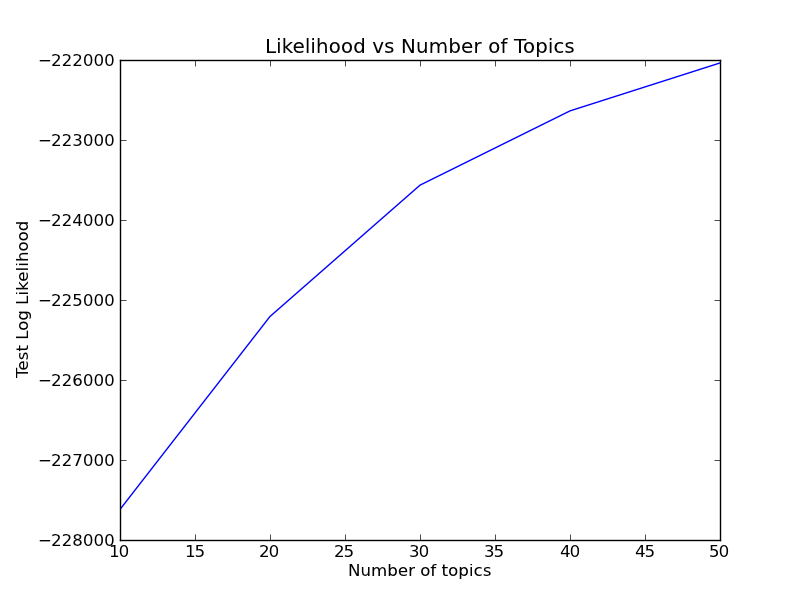
\includegraphics[scale=0.5]{../topics_plot}
				\end{center}
			\end{figure}
		\item
			\begin{figure}[H]
				\caption{Question 5}
				\begin{center}
					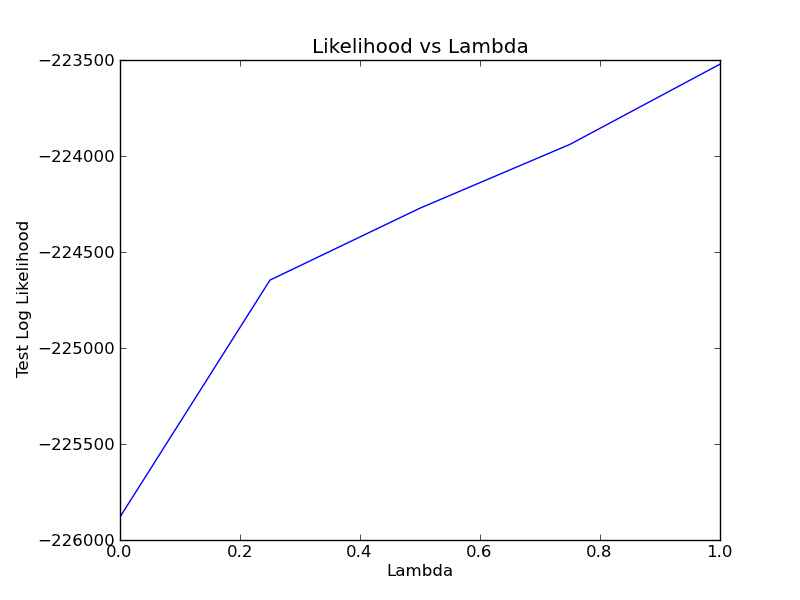
\includegraphics[scale=0.5]{../lambda_plot}
				\end{center}
			\end{figure}
		\item \begin{enumerate}
			\item Both conferences publish papers exclusively on statistical
			methods and other machine learning techniques. Naturally, from this
			there will arise a similarity between the global and local topics
			across each conference. However, we do see a difference between the 
			specificity between the global and local topics. 
			
			Among the global topics are a few that represent general machine
			learning concepts such as a ``feature'' topic which include
			``feature,'' ``extraction,'' ``classifier,'' ``hyperplane,'' as well as a ``modeling''
			topic which include words such as ``statistical'', ``probabilistic'', 
			``framework,''
			``entropy,'' ``model.'' In addition, we pick out a few topics that relate with
			topics that relate to all computer science conference papers. These
			include results, significant, new important. 
			
			On the local level, we see topics that very clearly belong to one or
			the other conference. In NIPS we see a reinforcement learning that includes
			``Markov,'' ``reinforcement,'' ``control,'' and 
			``decision.'' We also see a computational
			neural science and neural network topic with related words. The ACL
			clearly contains NLP related topics with topics related to parsing,
			SMT, IR, QA, and Semantics.
			
			\item 
			
			When the value for $\lambda$ is close to 0, this means that all of
			the topics come from the global corpus. The global topics are rather
			diverse as before. You can see topics that come from the NIPS
			and ACL corpora. These tend to be general machine learning topics.
			The corpus-specific topics are all the same. This is because none
			of the words are drawn from the corpus-specific topic, so each  of
			the words is equally likely. Therefore, all of the topics are the same.
			
			Then when $\lambda$ goes to 1, all of the global corpus topics
			are identical. This follows a similar argument as before. The NIPS
			and ACL topics are very specific to each group. The NIPS has topics
			about neural networks and imaging; the ACL topics deal with
			semantics and other NLP related topics. This is expected.
			
			\item As $\alpha$ goes to infinity, the Dirichlet from which every $\theta$ 
			will be sampled will become a point mass.
			In that extreme case, we should get
			every topic to be equally likely in each document, which will make it
			harder to associate individual topics with each document.
		\end{enumerate}
	\end{enumerate}
	
	\section{Variational Inference}
	\subsection{Analysis Questions}
	
	We toiled and troubled on this task writing many equations on the whiteboard and on paper. Below we've provided a simple derivation that skips over many steps. For a more detailed approach see the \texttt{variational.tex} file we've attached. We believe this is enough since it is roughly equivalent to the amount of work they showed in the original paper.
\\ \\

Notation: $w_n^v$ is an indicator variable that means the type of the $n$th word is $v$. $c_d^c$ means the corpus type of the $d$th document is $c$. This is very similar to the notation used in the paper. The subscripts have the following meaning $d$ = document index, $n$ = word token index $v$ = word type index , $g$ = global topic, $l$ = local topic $c$  = corpus id, $k$ = topic id.  Also note that $\log(\phi_{d,v,l,k,c})$ is a point estimate for expected value of the natural statistic of a Dirichlet (the difference of the two digammas) according to https://lists.cs.princeton.edu/pipermail/topic-models/2009-June/000560.html. 
We can now factorize $p$ and $q$ according to the graphical model
\\ \\
The upper bound on the likelihood.
$$
\mathcal{L}_{[\gamma,\delta,\epsilon,\psi; \alpha,\beta,\lambda]} = E_q\left[\log( p(\mathbf{\theta}|\alpha) p(\mathbf{w}|\mathbf{z},\mathbf{x},\mathbf{c},\mathbf{\phi}) p(\mathbf{c}) p(\mathbf{x}|\lambda) p(\mathbf{z}|\theta) p(\phi |\beta,\lambda )\right] - H_q\left[ \log(q(\mathbf{\theta}|\gamma) q(\mathbf{z}|\delta) q(\mathbf{x}|\epsilon) 	q(\phi|\psi)) \right] 
$$
\begin{multline*}
\mathcal{L}_{[\gamma,\delta,\epsilon,\psi; \alpha,\beta,\lambda]}  = E_q\left[\log( p(\mathbf{\theta}|\alpha)\right] + E_q\left[ \log(p(\mathbf{w}|\mathbf{z},\mathbf{x},\mathbf{c},\mathbf{\phi})\right] + E_q\left[ \log(p(\mathbf{c})\right] + E_q\left[ \log(p(\mathbf{x}|\lambda))\right] \\ + E_q\left[ \log(p(\mathbf{z}|\theta))\right]  + E_q \left[ \log(p(\phi |\beta ))\right] - E_q\left[ \log(q(\mathbf{\theta}|\gamma)) \right] - E_q\left[\log(q(\mathbf{z}|\epsilon))\right] - E_q\left[ \log( q(\mathbf{x}|\delta)) \right] - \\ E_q\left[ \log(	q(\phi|\psi)) \right] 
\end{multline*}

\section*{$\delta$}
$\delta$ is the variational parameter for $x$ and we need an update rule for it. 

$$
\mathcal{L}_{[\delta]} = \mathbb{E}_q\left[ \log(p(\mathbf{w}|\mathbf{z},x,c,\phi )) \right] + \mathbb{E}_q\left[\log(p(x|\lambda))\right] - \mathbb{E}_q\left[\log(q(x|\lambda))\right]
$$
We can expand this to (note that $T =\{\text{g,l}\}$
\begin{multline*}
\sum_{n=1}^{N_d} \sum_{k=1}^K \sum_{t=1}^T \;w_n^w c_d^c \;\delta_{d,t,n} \epsilon_{d,n,k} \log(\phi_{d,n,v,k,c}) + \sum_{n=1}^{N_d} \sum_{t=1}^T \delta_{d,t,n}\log(\lambda_t) \\ - \sum_{n=1}^{N_d}\sum_{t=1}^T \delta_{d,t,n}\log(\delta_{d,t,n}) + \zeta_n(\sum_{t=1}^T\delta_{d,t,n} - 1)
\end{multline*}
Now we take the partial for the global and local $\delta$ and $\zeta_i$ is a Lagrance multiplier.
$$
\frac{\partial}{\partial \delta_{d,g,n}}\left[ \mathcal{L}_{[\delta]}\right] = \sum_{k=1}^K \epsilon_{d,n,k} \log(\phi_{d,v,g,k,c}) + \log(\lambda_g) - \log(\delta_{d,g,n}) - \zeta_g
$$
Setting this equal to 0 and relocating the $\log(\delta){d,g,n}$ to the left hand size and then exponentiating yields.
$$
\delta_{d,g,n} \propto w_n^v \lambda_g \exp\left\{ \sum_{k=1}^K \epsilon_{d,n,k} \log(\phi_{d,v,g,k,c})  \right\}
$$
By analogy, we achieve the update rule for each local corpus
$$
\delta_{d,l,n} \propto  w_n^v c_n^c \lambda_l \exp\left\{ \sum_{k=1}^K \epsilon_{d,n,k} \log(\phi_{d,v,l,k,c})  \right\}
$$
Note that here we have treated $\lambda$ as a vector so $\lambda_g$ (global) = $\lambda$ (old notation) and $\lambda_l$ (local) = $(1 - \lambda)$. 
\section*{$\epsilon$}
$\epsilon$ is the variational parameter for $\theta$. We get
$$
\mathcal{L}_{[\epsilon]} =  \mathbb{E}_q\left[ \log(p(\mathbf{w}|\mathbf{z},x,c,\phi)) \right] + \mathbb{E}_q\left[\log(p(\mathbf{z}|\theta))\right] - \mathbb{E}_q\left[\log(q(\mathbf{z}|\epsilon))\right] 
$$
Now since we are clever, we note that the only difference between this and the $\mathcal{L}_{[\phi]}$ in Blei et al. (2003) is $\mathbb{E}_q\left[ \log(p(\mathbf{w}|\mathbf{z},x,c,\phi)) \right]$. Thus we can simply write down adapation of equation (16) to include the $\delta$ term.
$$
\epsilon_{d,n,k} \propto \exp\left\{\sum_t^T w_n^v c_n^c \; \delta_{d,t,n} \log(\phi_{d,v,l,k,c}) + \Psi(\gamma_{dk}) 
\right\}
$$
\section*{$\phi$}
Finally to get the updates for $\phi$ we look at A.4.1 in Blei et al. (2003). We notice that only addition will be $\delta_{d,t,n}$ which will be constant with respect to the derivative. So we can write down by inspection the global update
$$
\phi_{d,v,g,k} \propto \beta + \sum_{d=1}^D\sum_{n=1}^{N_d} w_{d,n}^v \; \delta_{d,g,n} \epsilon_{d,n,k}
$$
Now to get the local update, we have
$$
\phi_{d,v,l,k,c} \propto \beta +  \sum_{d=1}^D\sum_{n=1}^{N_d} w_{d,n}^v c_{d}^c\; \delta_{d,l,n} \epsilon_{d,n,k}
$$
The updates for $\gamma$ are identical. I repeat them for the sake of repeating them but this is extremely straight forward since no part of the model has changed.
$$
\gamma_{dk} = \alpha + \sum_{n=1}^{N_d} \epsilon_{d,n,k}
$$ 
	
	\setcounter{subsection}{2}
	\subsection{Empirical Questions}
	\begin{enumerate}
		\item 
		\item
		\item
		\item
	\end{enumerate}

\end{document}
